\section{Introduction}\label{sec:introduction}
\mycite{Fanger1970} developed the \ac{pmv} model, which is now incorporated into the \gls{7730} Standard~\cite{iso7730} in its original form.
The \ac{pmv} is an index that aims to predict the mean value of the thermal sensation votes (self-reported perceptions) of a large group of people on a sensation scale expressed from \num{-3} to \num{3} corresponding to the categories ``cold,'' ``cool,'' ``slightly cool,'' ``neutral,'' ``slightly warm,'' ``warm,'' and ``hot.''~\cite{iso7730, ashrae552023}.
The \ac{pmv} model has been widely used worldwide by researchers and practitioners.
It is the most extensively used thermal comfort index for estimating thermal sensation.
A search within the article title, abstract, and keyword on Scopus with the search term ``predicted mean vote'' returns approximately \num{2050} documents.
Out of those \num{1200} are scientific peer-reviewed articles published in the research area of engineering, environmental science, social sciences, and energy.
This highlights this model's extensive adoption and use among the scientific community.
To this date, the \ac{pmv} remains to be the most utilized thermal comfort model even though several studies have highlighted that the \ac{pmv} has low accuracy in predicting thermal sensation votes~\cite{Cheung2019, Yao2022, kim2019thermal, tartarini2018thermal, Humphreys2002, doherty_evaluation_1988, tartarini_prediction_2023}.

To overcome the accuracy concerns, in particular when high air speed is used to cool people, the \gls{55} Standard uses a modified version of the original model, the \ac{pmv-ce}~\cite{ashrae552023}.
The best source to see how \ac{pmv-ce} works is the Standard itself, but the Standard does not explain why some choices were implemented.
A partial justification of the model is described in \mycite{arens_moving_2009} and \mycite{yang_cooling_2015}.
The process used to calculate the \ac{pmv-ce} in the \gls{55} is summarized in the flowchart depicted in Figure~\ref{fig:flowchart_pmv_ce}.
\begin{figure}[!htb]
    \centering
    \begin{tikzpicture}[node distance=1cm and 3cm, transform shape]
        \node (start) [startstop] {\acs{pmv} calculation as per \gls{55}};
        \node (dec1) [decision, below of=start, yshift=-.25cm] {\acs{met} $> \qty{1}{met}$ };
        \node (pro1a) [process, right of=dec1, xshift=3.5cm] {\acs{v} = \acs{v}$+ 0.3 ($\acs{met}$-1)$};
        \node (dec2) [decision, below of=dec1, yshift=-0.75cm] {\acs{met} $> \qty{1.2}{met}$ };
        \node (pro2a) [process, right of=dec2, xshift=3.5cm] {\acs{clo} = \acs{clo}$(0.6 + 0.4/$\acs{met}$)$};
        \node (dec3) [decision, below of=dec2, yshift=-0.75cm] {\acs{v} $> \qty{0.1}{\m\per\s}$ };
        \node (end1) [startstop, below of=dec3, yshift=-.25cm, xshift=-4cm] {\acs{pmv}(\acs{tdb}, \acs{tr}, \acs{rh}, \acs{v}, \acs{met}, \acs{clo})};
        \node (pro3) [process, below of=dec3, yshift=-.25cm, xshift=3cm] {Calculate \acs{ce}};
        \node (end2) [startstop, below of=pro3, yshift=-.5cm] {\acs{pmv}(\acs{tdb} - \acs{ce}, \acs{tr} - \acs{ce}, \acs{rh}, \acs{v} = \qty{0.1}{\m\per\s}, \acs{met}, \acs{clo})};

        \draw [arrow] (start) -- (dec1);
        \draw [arrow] (dec1) -- node[above,pos=0.3] {Yes} (pro1a);
        \draw [arrow] (dec1) -- node[right,pos=0.3] {No} (dec2);
        \draw [arrow] (pro1a) -- ($(pro1a.south)+(0,-0.5)$) -| (dec2);
        \draw [arrow] (dec2) -- node[above,pos=0.3] {Yes} (pro2a);
        \draw [arrow] (dec2) -- node[right,pos=0.3] {No} (dec3);
        \draw [arrow] (pro2a) -- ($(pro2a.south)+(0,-0.5)$) -| (dec3);
        \draw [arrow] (dec3) -- ($(dec3.west)$) -| node[above,pos=0.3] {No} (end1);
        \draw [arrow] (dec3) -- ($(dec3.east)$) -| node[above,pos=0.3] {Yes} (pro3);
        \draw [arrow] (pro3) -- (end2);
    \end{tikzpicture}
    \caption{Flowchart depicting the steps for the calculation of the PMV following the \gls{55} Standard.}
    \label{fig:flowchart_pmv_ce}
\end{figure}
In summary, when the \ac{v} exceeds \qty{0.1}{\m\per\s} the \gls{55} prescribes the use of the \ac{ce}.
The reader should note that \ac{v} is not the measured value.
The value of \ac{v} measured by the sensors, should be adjusted based on the \ac{met} of the occupant if \ac{met}~$>$~\qty{1}{met} using this equation \ac{v} = \ac{v}$+ 0.3 ($\ac{met}$-1)$.
The value of \ac{ce} is calculated using the \ac{set} equation.
The \ac{ce} is then subtracted from both the \ac{tdb} and \ac{tr}.
The resulting values become the new inputs in the \ac{pmv} model.
Since the \ac{ce} accounts for  convective heat losses from the person to its environment the value of \ac{v}, used to calculate the \ac{pmv}, is set to \qty{0.1}{\m\per\s}.
The other three input parameters (\ac{clo}, \ac{rh}, \ac{met}) remain unchanged.
Consequently, for a given thermal environment, results of the two \ac{pmv} formulations differ only when the value of \ac{v} is higher than \qty{0.1}{\m\per\s}.
To show to the reader by how much the output of the two models differ, we calculated the comfort regions ($\mid$\ac{pmv}$\mid \leq 0.5$) for different values of \ac{v} using the \ac{pmv} and \ac{pmv-ce} models assuming \ac{met}~=~\qty{1.2}{met} and \ac{clo}~=~\qty{0.5}{clo}.
We plotted the results in Figure~\ref{fig:comfort_regios_pmv_pmvce}.
\begin{figure}[!htb]
    \centering
    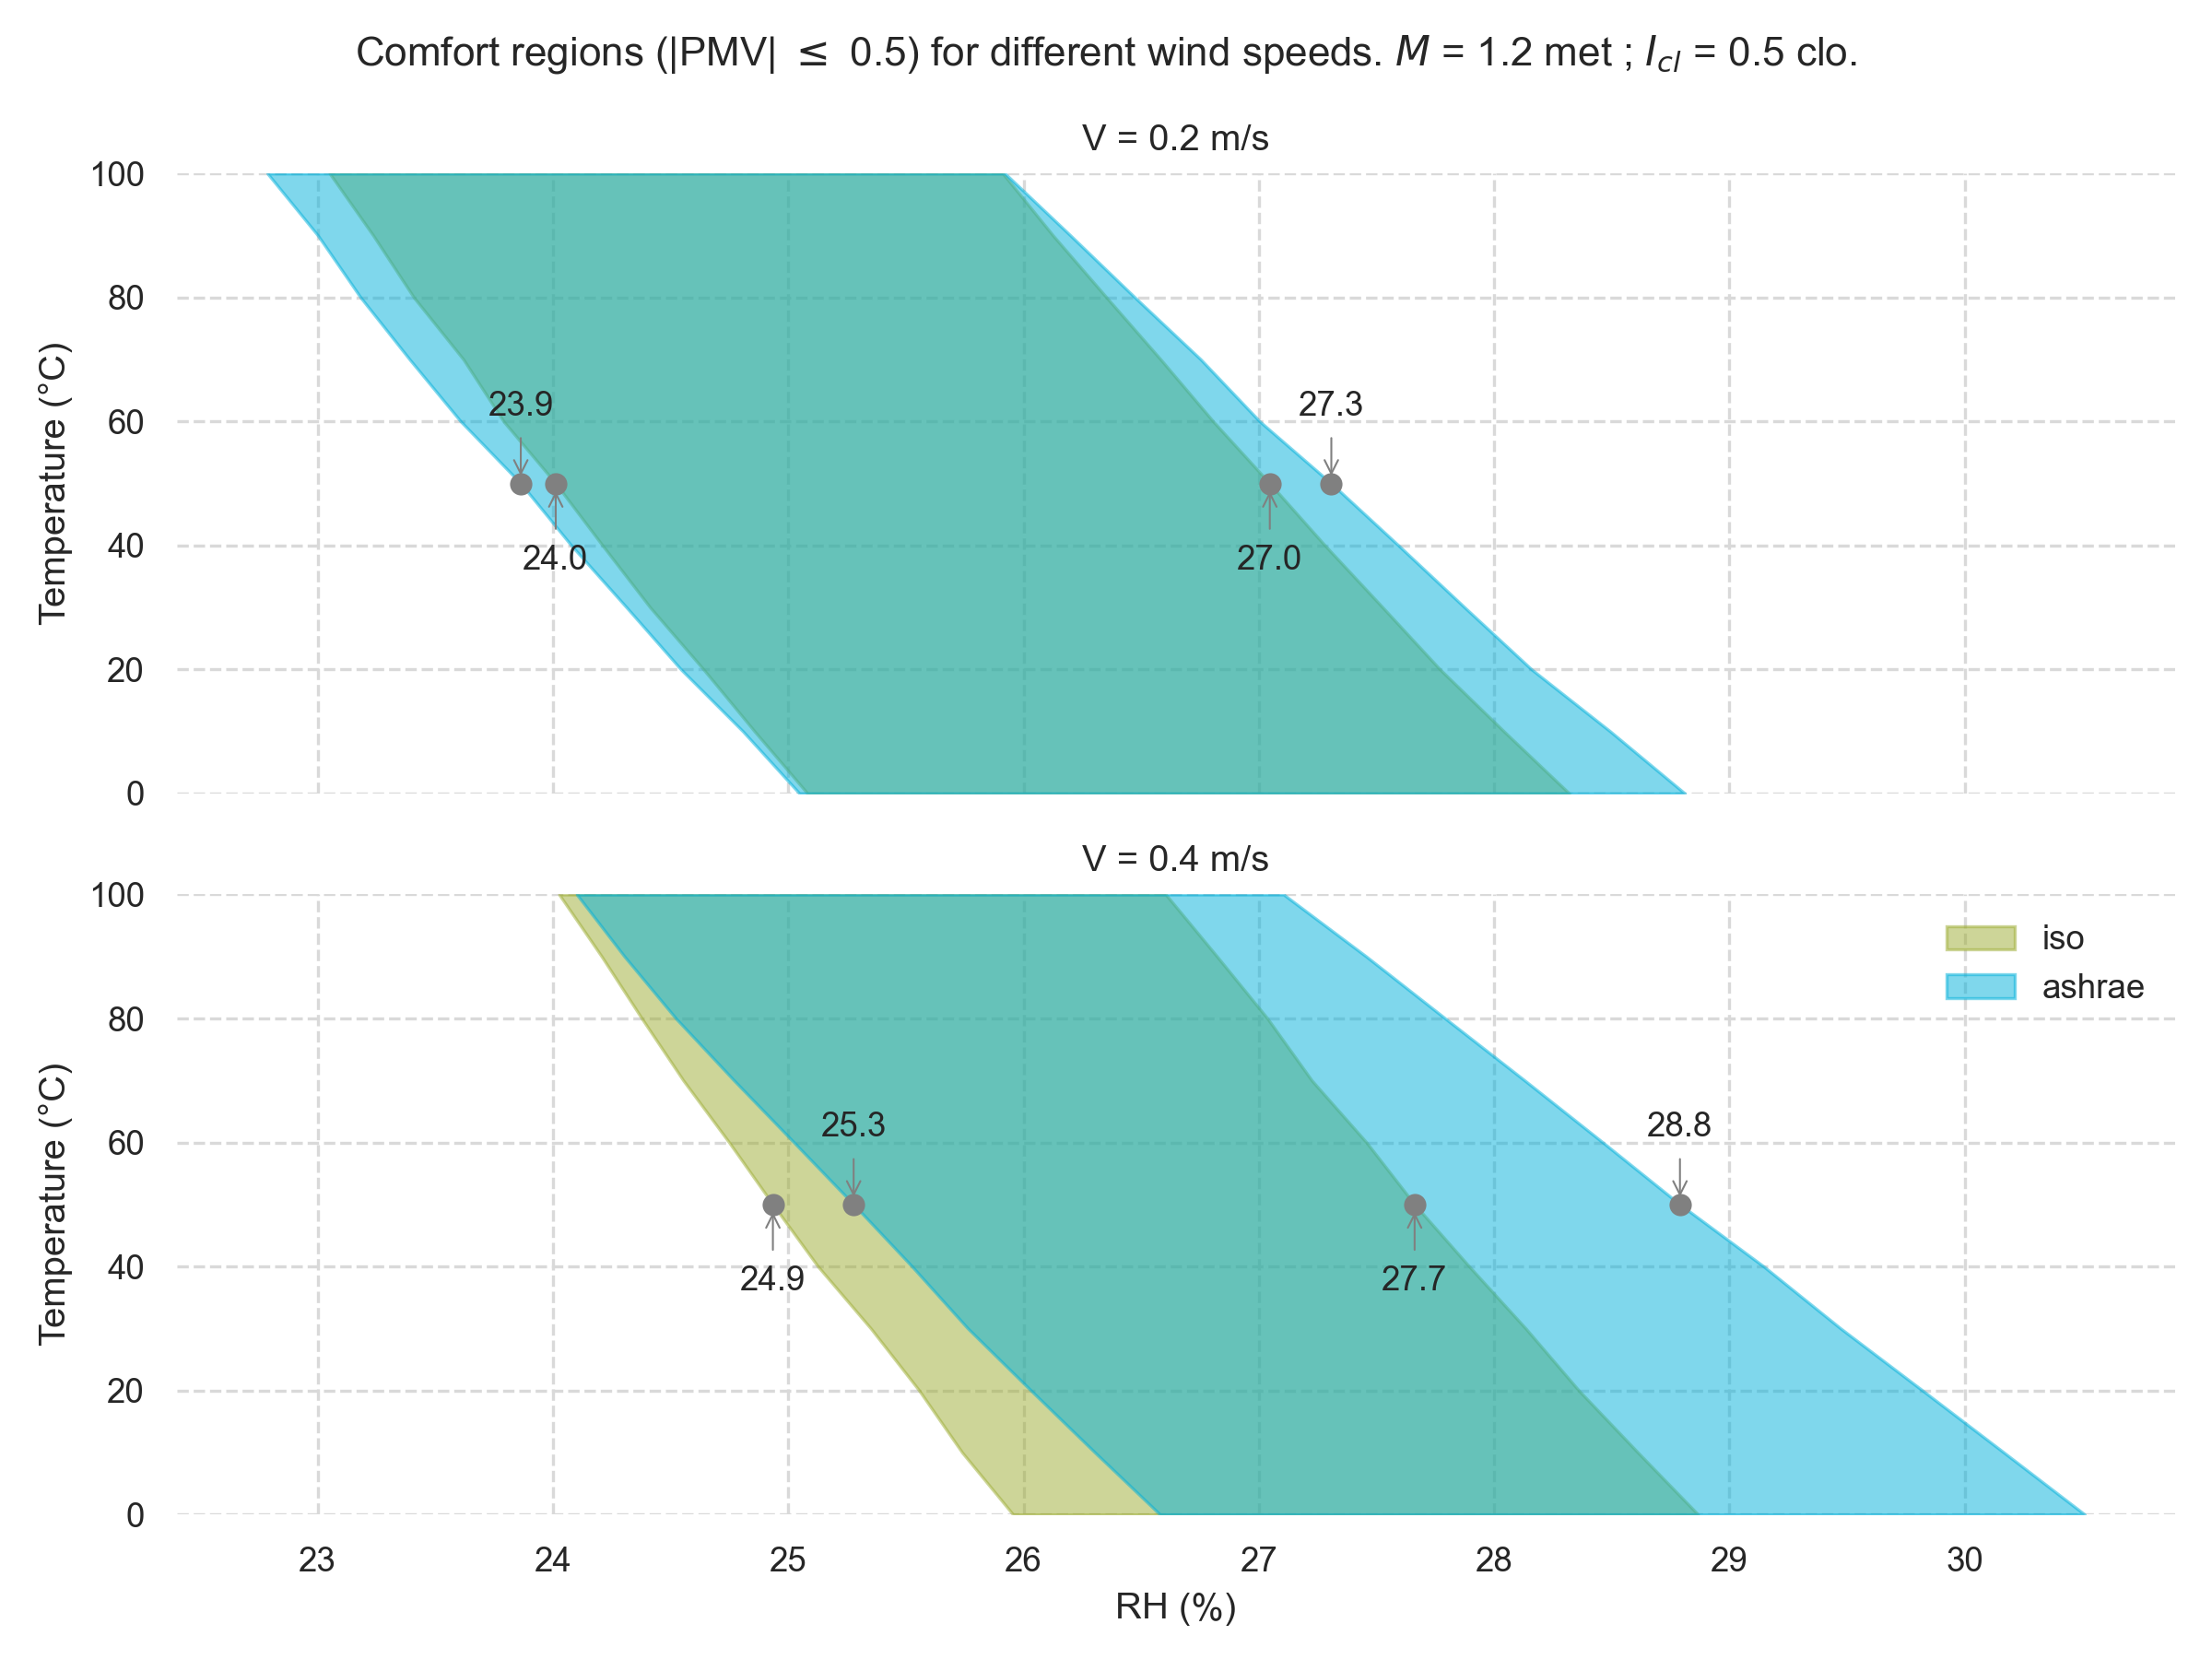
\includegraphics[width=1\textwidth]{figures/pmv_comfort_regions}
    \caption{Comfort regions ($|$\ac{pmv}$|$~$\leq$~\num{0.5}) calculated using \ac{pmv} and \ac{pmv-ce} models.
    The chart shows how the comfort regions change as a function of \ac{v}.
    We assumed $M$~=~1.2 met, $i_{cl}$~=~0.5 clo.
    \label{fig:comfort_regios_pmv_pmvce}}
\end{figure}
The results show that for \ac{v}~=~\qty{0.4}{\m\per\s} the comfort regions estimated using the \ac{pmv-ce} is wider than the one calculated using the \ac{pmv} and shifted towards the warmer temperatures.

The rationale for using the \ac{pmv-ce} model is that the original \ac{pmv} formulation cannot accurately estimate latent and sensible heat losses from the skin to the environment when \ac{v}~$>$~\qty{0.1}{\m\per\s}.
However, this method has its own limitations.
First, it should be noted that over the years, the critical value of \ac{v} has been changed, from \qty{0.15}{\m\per\s} in \mycite{Schiavon2014} to \qty{0.2}{\m\per\s} in the ASHRAE 55--2017~\cite{ASHRAE552017, arens_moving_2009} to \qty{0.1}{\m\per\s} in \gls{55}~\cite{ashrae552023}.
Second, calculating the \ac{pmv-ce} is more computationally intensive and complex since it requires the user to solve two heat balance equations, the \ac{pmv} and the two-node model.
Third, we could not find any peer-reviewed scientific publication that quantified the accuracy improvements of this model over the original \ac{pmv}.
Finally, the \ac{set} temperature which is used to calculate the \ac{ce}, is defined as the hypothetical isothermal environment at a \ac{rh} of \qty{50}{\percent}, \ac{v}~$\leq$~\qty{0.1}{\m\per\s}, and \ac{tr}~=~\ac{tdb} in which the total heat loss from the skin of an imaginary occupant wearing clothing, standardized for the activity concerned, is the same as that from a person in the actual environment with actual clothing and activity level~\cite{ashrae552023}.
However, while \ac{v}, used to calculate the \ac{pmv-ce}, is set to \qty{0.1}{\m\per\s} since the \ac{ce} already accounts for the convective heat losses, the value of \ac{rh} and \ac{clo} are not adjusted to compensate for the fact that \ac{set} normalizes them.
We could not find a rationale for this choice in the available literature.

Several other formulations of the \ac{pmv} model have been proposed to complicate this issue further.
Among the most notable formulations there are the: \ac{pmvs}~\cite{GaggeSET}, \ac{pmvg}~\cite{GaggeSET}, \ac{epmv}~\cite{Toftum2002}, and \ac{athb}~\cite{Schweiker2022}.
\mycite{Yao2022} provides a comprehensive review of different thermal comfort models and compares and describes some of the above-mentioned models.
Here, we decided to focus on the \ac{pmv} and \ac{pmv-ce} models since they are the most widely used thermal comfort models worldwide and are incorporated in the \gls{7730} and \gls{55} Standards.

Choosing between the \ac{pmv} and \ac{pmv-ce} is consequently now a source of confusion for many practitioners, educators, and researchers worldwide since both models are widely adopted and incorporated in many building codes and standards worldwide.

%In 2002, Fanger, P. O. and Toftum, J. developed the \ac{epmv} an extension of the \ac{pmv}.
%The \ac{epmv} includes an expectancy factor introduced for use in non-air-conditioned buildings in warm climates.
%The authors argued that people adapt to the warm environment by decreasing their \ac{met} rate.
%They, consequently, propose to reduce the metabolic rate used to calculate the \ac{pmv} by \qty{6.7}{\percent} for every scale unit of \ac{pmv} above neutral.
%The resulting \ac{pmv} value is multiplied by the \ac{ef}.
%The \ac{ef} for non-air-conditioned buildings can be determined by the length of warm weather throughout the year and whether such buildings may be compared to many others in the region that are air-conditioned.
%If the temperature is hot all year or most of the year and there are no or few other air-conditioned buildings, \ac{ef} may be \num{0.5}, but if there are many other air-conditioned buildings, \ac{ef} may be \num{0.7}.
%For non-air-conditioned buildings in locations where the temperature is warm solely during the summer and no or few buildings have air-conditioning \ac{ef} is \numrange{0.7}{0.8}, whereas it is \numrange{0.8}{.9} in areas where there are numerous air-conditioned buildings.
%In regions with only brief periods of warm weather during the summer, the expectancy factor may be \numrange{0.9}{1}.
%This arbitrary and non-scientific definition of the expectancy factor makes the \ac{epmv} difficult to calculate and non-generalizable.
%Consequently, the \ac{epmv} has not gained any widespread adoption.
%
%Yao, R. et al. (2009) developed the Adaptive Predicted Mean Vote Model~\gls{apmv} to account for occupants adaptation.
%They used a ``Black Box'' model to estimate an adaptive coefficient which is in turn used to calculate the \gls{apmv} using the following equation: $\mathrm{aPMV} = \mathrm{PMV}/(1+\lambda \mathrm{PMV})$
%The main issue with this approach is that the adaptive coefficient cannot be known a priori, but it is estimated based on the \ac{tsv} collected by a cohort of participants.
%This approach cannot be, therefore, generalizable and similarly to the \ac{epmv} model the \gls{apmv} is rarely used in thermal comfort research.
%

\subsection{Comparison of ISO and ASHRAE PMV formulations}\label{subsec:comparision-of-pmv-formulations}
To our knowledge, no previous study compared in detail the accuracy of the \ac{pmv} and \ac{pmv-ce} models, which are used in the \gls{7730} and \gls{55} Standards.
Some notable works that tried to determine the accuracy of the \ac{pmv} model include the manuscript from \mycite{doherty_evaluation_1988} who evaluated the ability of the \ac{pmv} and \ac{set} models to predict several physiological variables (i.e., skin temperature, core temperature, and skin wettedness) under a wide range of still air environments and metabolic rates.
They concluded that the \ac{pmv} model is accurate for simulations of resting subjects, but its accuracy decreases as a function of metabolic rate.
Humphreys and Nicol estimated the effects of measurement and formulation error on predicting thermal sensation using the \ac{pmv}~\cite{Humphreys2000}.
They used the ASHRAE Global Thermal Comfort database I and determined that the measurement error and the error introduced by the \ac{pmv} model formulation had a similar and non-negligible contribution.
They also determined the validity of the \ac{pmv} for predicting comfort votes collected in field studies~\cite{Humphreys2002}.
They concluded that the \ac{pmv} range of applicability should be significantly reduced and it fails to predict the extent of thermal dissatisfaction of people in buildings.
The \ac{pmv} was free from bias only when it was used to predict thermal neutrality~\cite{Humphreys2002}.
\mycite{Cheung2019} determined the accuracy of the \ac{pmv} model, by comparing its results with the \ac{tsv} from the ASHRAE Global Thermal Comfort Database II.
They found that the thermal sensation predicted by the PMV model, on average, is one full thermal sensation scale unit away from the subject’s responses, confirming the results of~\mycite{Humphreys2002}.
\mycite{Cheung2019} also concluded that the accuracy of \ac{pmv} was only \qty{34}{\percent}, the model has a slightly higher prediction accuracy for sensation close to neutrality, but the accuracy declined towards either end of the thermal sensation scale, and it overestimated both hot and cold sensations.
They also found that the Predicted Percentage of Dissatisfied (PPD) failed to predict the percentage of unacceptable votes if the thermal sensation was predicted using the PMV model and suggested its removal from \gls{55} Standards.
These results were confirmed based on the Chinese Thermal Comfort database~\cite{du_evaluation_2022}.
\mycite{Yao2022} compared the \ac{pmv} and \ac{pmv-ce} models, however, their aim was primarily to compare these two formulations with other adaptive \ac{pmv} formulations, hence, they do not provide a detailed analysis on the prediction accuracy of the two models.
They focus significantly on how the models perform in different climates and when applied to people from different world regions and their analysis only reports the mean bias of the different models.
This, as depicted by \mycite{Humphreys2000}, does not provide sufficient insights and information in determining which model is more accurate since it does not explain how the model performs over a wide range of environmental, personal conditions, and \ac{tsv}.
Reporting the classification accuracy of the \ac{pmv} formulations when people are grouped by their \ac{tsv} is particularly important for an unbalanced dataset like the \ac{db2} where most of the participants reported to be `neutral'.
Finally, \mycite{Yao2022} only reported the overall bias for the whole dataset, even though the two formulations only differ when the \ac{v} exceeds \qty{0.1}{\m\per\s}.
\mycite{tartarini_prediction_2023} concluded that the \ac{pmv} and \ac{pmv-ce} models accuracy is \qty{35}{\percent} and \qty{36}{\percent} for $\mid$\ac{pmv}$\mid \leq 2$, \qty{43}{\percent} and \qty{44}{\percent} for $\mid$\ac{pmv}$\mid \leq 1$ in predicting the self-reported thermal sensation of people, respectively.
However, their analysis is limited to providing the precision of the model alone, without reporting the sensitivity (also commonly referred to as recall) and they do not provide the bias of the two models.

\subsection{Aim and Objectives}\label{subsec:aim-and-objectives}
In this paper, we compare the accuracy of the \ac{pmv} and \ac{pmv-ce} models used in the \gls{7730} and \gls{55} Standards, respectively.
The paper objective is to quantitatively answer the following questions:
which model should you use?
Which model is more accurate?
We used the self-reported \ac{tsv} recorded in the \acf{db2}.
We aim to determine which \ac{pmv} model is most accurate and which are its applicability limits.
This will allow \ac{pmv} users - engineers, architects, and educators - to make an informed decision on which model they should use and will help policymakers to select the most appropriate model to be used in Standards.